\documentclass{article}
\usepackage[utf8]{inputenc}
\usepackage{graphicx}
\usepackage{amsmath,amssymb}
\usepackage{amsthm}
\DeclareMathOperator{\argmax}{argmax}
\DeclareMathOperator{\argmin}{argmin}
\setlength\parindent{0pt}
\setlength{\topmargin}{-3cm}
\setlength{\textheight}{24cm}

% ready for submission
\usepackage[final]{neurips_2023}
\usepackage[utf8]{inputenc} 
\usepackage[T1]{fontenc}    
\usepackage{hyperref}       
\usepackage{url}            
\usepackage{booktabs}       
\usepackage{amsfonts}       
\usepackage{nicefrac}       
\usepackage{microtype}
\usepackage{hyperref}
\usepackage{xcolor}         
\usepackage{algpseudocode}
\usepackage{algorithm}
\usepackage{caption}
\usepackage{graphicx}
\usepackage{url}
\usepackage{subcaption}

\newlength\myindent
\setlength\myindent{2em}
\newcommand\bindent{%
  \begingroup
  \setlength{\itemindent}{\myindent}
  \addtolength{\algorithmicindent}{\myindent}
}
\newcommand\eindent{\endgroup}


\title{Final Report of DM887 Course Project}

\author{%
  Jiawei Zhao, Kristóf Péter\\
  Department of Mathematics and Computer Science\\
  University of Southern Denmark\\
  Moseskovvej, 5230 Odense \\
  \texttt{jizha22@student.sdu.dk} \\
  \texttt{krpet24@student.sdu.dk} \\
}


\begin{document}
\maketitle
\clearpage

\begin{abstract}
To implement the project \textbf{Learning to play Atari games with Bayesian Deep Expected SARSA}, we used \cite{BDQN} implemented according to \cite{EEtBDQN} as a theoretical baseline. The $Q$ used to determine the policy for each action are calculated as the matrix product of the output of a feature extractor in the form of a convolutional neural network, and a randomly generated Gaussian matrix representing the policy Q-weights to calculate the $Q$ from extracted features per permissible action. The feature extractor is updated by gradient descent, while the policy Q-weights are updated by a Bayesian posterior update based on a large number of sampled tuples representing the explored states, actions, next actions, and rewards. The large number of tuples sampled from the replay memory are used to simulate the observations in the posterior probability. In our algorithm, we use the expected $Q$ of the next states to calculate the Bellman values, instead of the maximum $Q$ per action at a $Q$ table during the gradient descent and update of policy Q-weights, which is the case in standard Q-learning.
\end{abstract}

\section{List of symbols and constants used as default values during training:}
\begin{enumerate}
    \item\textbf{Global variables:}
    \begin{enumerate}
        \item$env$ :  An Atari Game environment using RGB images to represent its states, which an agent interacts with, e.g., $env1$: \textit{ALE/Breakout-v5}, and $env2$: \textit{ALE/Pong-v5} from Gymnasium \cite{Gym}. We assign the set of all the aforementioned Atari Game environments as $ENV$.
        \item$reset$ : A statement setting the current $env \in ENV$ to its starting state, represented by a frame $fr$.
        \item$A$ : The action space of $env \in ENV$ with $A = \{0,1,2,\dots,|A-1|\}$ in $env \in ENV$ which we tested.
        \item$fr$ : A raw frame generated by $env \in ENV$ with a shape (210, 160, 3), representing an RGB image in $env \in ENV$ which we tested.
        \item$tfr$ : A transformed frame to the desired shape during pre-processing with a shape (84, 84), representing a grayscale image.
        \item$|A|$ : Size of $A$ in $env \in ENV$ which we tested.
        \item$FR_{skipped} = 4$ : Number of frames skipped (we step with the same action for this many frames).
        \item$t_{total}$ : Count of time steps passed during the algorithm at $env \in ENV$.
    \end{enumerate}
    \item\textbf{Neural Network parameters and $Q$ calculation:}
    \item\begin{enumerate}
        \item$4$ : Size of the input channels to the first convolutional layer, i.e., the number of stacked frames at the state tensor $s$.
        \item$512$ : Length of the output layer of the last fully connected linear layer, i.e., the number of features at the output tensor of $\phi(s)$.
        \item$\phi$ : Policy Network.
        \item$\theta$ : Weights of $\phi$.
        \item$\phi_{target}$ : Target Network.
        \item$\theta_{target}$ : Weights of $\phi_{target}$.
        \item$M$ : A matrix of mean vectors for generating from the multivariate normal distribution with shape $(|A|, 512)$.
        \item$M_a$ : A mean vector with shape $(512)$, which is an element of $M$ representing $a \in A$.
        \item$\Sigma$ : A tensor containing covariance matrices for generating the multivariate normal distribution with shape $(|A|, 512, 512)$.
        \item$\Sigma_a$ : A covariance matrix with shape $(512,512)$, which is an element of $Cov$ representing $a \in A$.
        \item$L$ : A tensor containing matrices of coefficients to generate from the normal distribution, calculated from $\Sigma$.
        \item$L_a$ : A matrix of coefficients to generate from the normal distribution, $L$ representing $a \in A$, calculated from $\Sigma_a$.
        \item$W$ : A matrix of random vectors generated from the multivariate normal distribution with shape $(|A|, 512)$.
        \item$W_a$ : A vector of $W$ with shape $(512)$, representing $a \in A$.
        \item$\phi\phi^T$ and $\phi_Y$ : Assistant variables used during a posterior update.
    \end{enumerate}
    \item\textbf{Replay Memory elements:}
    \begin{enumerate}
        \item$RM$ : Replay Memory, we store ($s$, $a$, $r$, $s'$, $a'$) tuples each representing a time step $t$ here.
        \item$B$ : A Batch of tuples from the replay memory
        \item$|B|$ : Batch size
        \item$s$: A state tensor with shape $(4,84,84)$, concatenated by $tfr_1, tfr_2, tfr_3, tfr_4$, which are pre-processed frames from four adjacent time steps. $(1,4,84,84)$ is the shape of which is fed into $\phi$ or $\phi_{target}$.
        \item$s'$: A tensor representing the next state, represents state which $env \in ENV$ moves to. $s'$ is constructed and shaped in an identical manner as $s$.
        \item$a$ : An action $a \in A$ represented by an index in integer defined by $A$ in $env \in ENV$)
        \item$r$ or $reward$: A reward represented by an integer or a float in $env \in ENV$.
        \item$\sum{r'}$ : The cumulative reward collected by skipping frames performed during the frame-skipping option.
        \item$a'$ : A boolean value indicating whether $t$ terminates the episode $e$ which $t$ belongs to after $s'$.
        \item$B_s$ : A batch of states with shape $(|B|,4,84,84)$.
        \item$B_{s'}$ : A batch of next states with shape $(|B|,4,84,84)$.
        \item$B_a$ : A batch of actions with shape $(|B|)$.
        \item$B_r$ : A batch of rewards with shape $(|B|)$.
        \item$B_{a'}$ : A batch of done values with shape $(|B|)$.
    \end{enumerate}
    \item\textbf{Constants(unchanged throughout the algorithm):}
    \begin{enumerate}
        \item$|RM|=200000$ : Size of the Replay Memory.
        \item$F_1=1000$ : Thompson sampling frequency .
        \item$F_2=4$ : Training frequency.
        \item$F_3=10000$ : Target update frequency.
        \item$F_4=10$ : Posterior update frequency beyond $F_3$.
        \item$B_{gd}=32$ : Training update batch size .
        \item$B_{post}$ : Posterior update batch size.
        \item$LR=0.0025$ : Learning rate for the optimizer.
        \item$\gamma=0.99$ : Learning rate for the Bellman equation
        \item$N=10000$: Maximum number of episodes to run the algorithm. An episode takes place between the initial state and the final state of the environment.
        \item$\sigma = 0.001$ Prior variance
        \item$\sigma_n = 1$ Noise variance
        \item$I$ : Identity matrix
    \end{enumerate}
    \item\textbf{Functions:}
    \begin{enumerate}
        \item$MSE(\cdot,\cdot)$ : The mean squared error (MSE) function used for loss calculation taking two vectors as inputs.
        \item$Adam(\cdot,LR,\theta)$ : The optimizer used for updating the weights of a neural network's weights by gradient descent. The input parameters represent the loss by a scalar tensor with gradient information, the learning rate, and weights of the $\phi$ respectively.
        \item$Cholesky(\cdot)$ : The Cholesky factorization decomposing a symmetric, positive-definite matrix $X$ which suffices $X =YY^T$, returns $Cholesky(X) = Y$. It is used for calculating the coefficient vectors in the multivariate normal distribution from its covariance matrix.
        \item$Softmax(\cdot)$ : Calculates a vector of probabilities (positive numbers summing to 1) from a vector of numbers, using the softmax function.
    \end{enumerate}
    \item\textbf{Other:}
    \begin{enumerate}
        \item $\mathcal{N}(M_a,\Sigma_a)$ Multivariate normal distribution with means $M_a$, covariance matrix $\Sigma_a$
    \end{enumerate}
\end{enumerate}

\section{Bayesian Q-factor network design}
We used a convolutional neural network structure to extract the features from the frames created in the Gymnasium Atari environments \cite{Gym}. Using the same structure as explained below, we will define a Policy Network as $\phi$ and a Target Network as $\phi_{target}$ for feature extraction. However, the $Q$ used in the action selection (policy) are going to be given by
\[W_a \sim \mathcal{N}(M_a,\Sigma_a) : \; a=0,1,2,\dots,|A|\]
\[Q(s) = W^T\phi(s).\]
\[Q(s,a) = W_a^T\phi(s).\]
Making our randomly generated $W_a$ vectors a sort of last Bayesian Layer. The parameters $M_a,\;\Sigma_a$ are going to be updated by Bayesian inference based on the explored states during the Posterior Update step.

\subsection{Input Structure:}
 The frames $fr$ come in the form of $(210, 160, 3)$ colored images, however, during pre-processing we turn them into size $(84,84)$ grayscale images $tfr$. A singular input for the network will be referred to as a $s$, with shape $(4,84,84)$, that consists of $4$ concatenated, pre-processed $fr$ frames of shape $(84,84)$. In case we want to have a batch of states as input, it will be of shape $(|B|,4,84,84)$, consisting of $|B| = B_{gd}$ number of $s$.
\subsection{Network Structure:}

\begin{algorithmic}[H]

\State The number of in-channels of the first layer will be the number of frames in the frame stack which we refer to as $state$, therefore $4$ in our case.
\State The length of the output of the last layer (fully connected linear layer), will be a chosen number for the feature vector length, therefore, $512$ in our case.
\State These and the other channels are as follows:
\State \textbf{First convolutional layer (input):} $(4, 32)$ with a kernel size $8$ and stride $4$
\State Batch Normalization for the output of layer 1
\State \textit{ReLU} activation
\State \textbf{Second convolutional layer (hidden):} $(32, 64)$ with a kernel size $4$ and stride $2$
\State Batch Normalization for the output of layer 2
\State \textit{ReLU} activation
\State \textbf{Third convolutional layer (hidden):} $(64, 64)$ with a kernel size $3$ and stride $1$
\State Batch Normalization for the output of layer 3
\State \textit{ReLU} activation
\State \textbf{Fully-connected linear layer (output):} $(7\cdot7\cdot32\cdot2,512)$
\State \textit{ReLU} activation

\end{algorithmic}

\begin{figure}[H]
    \centering
    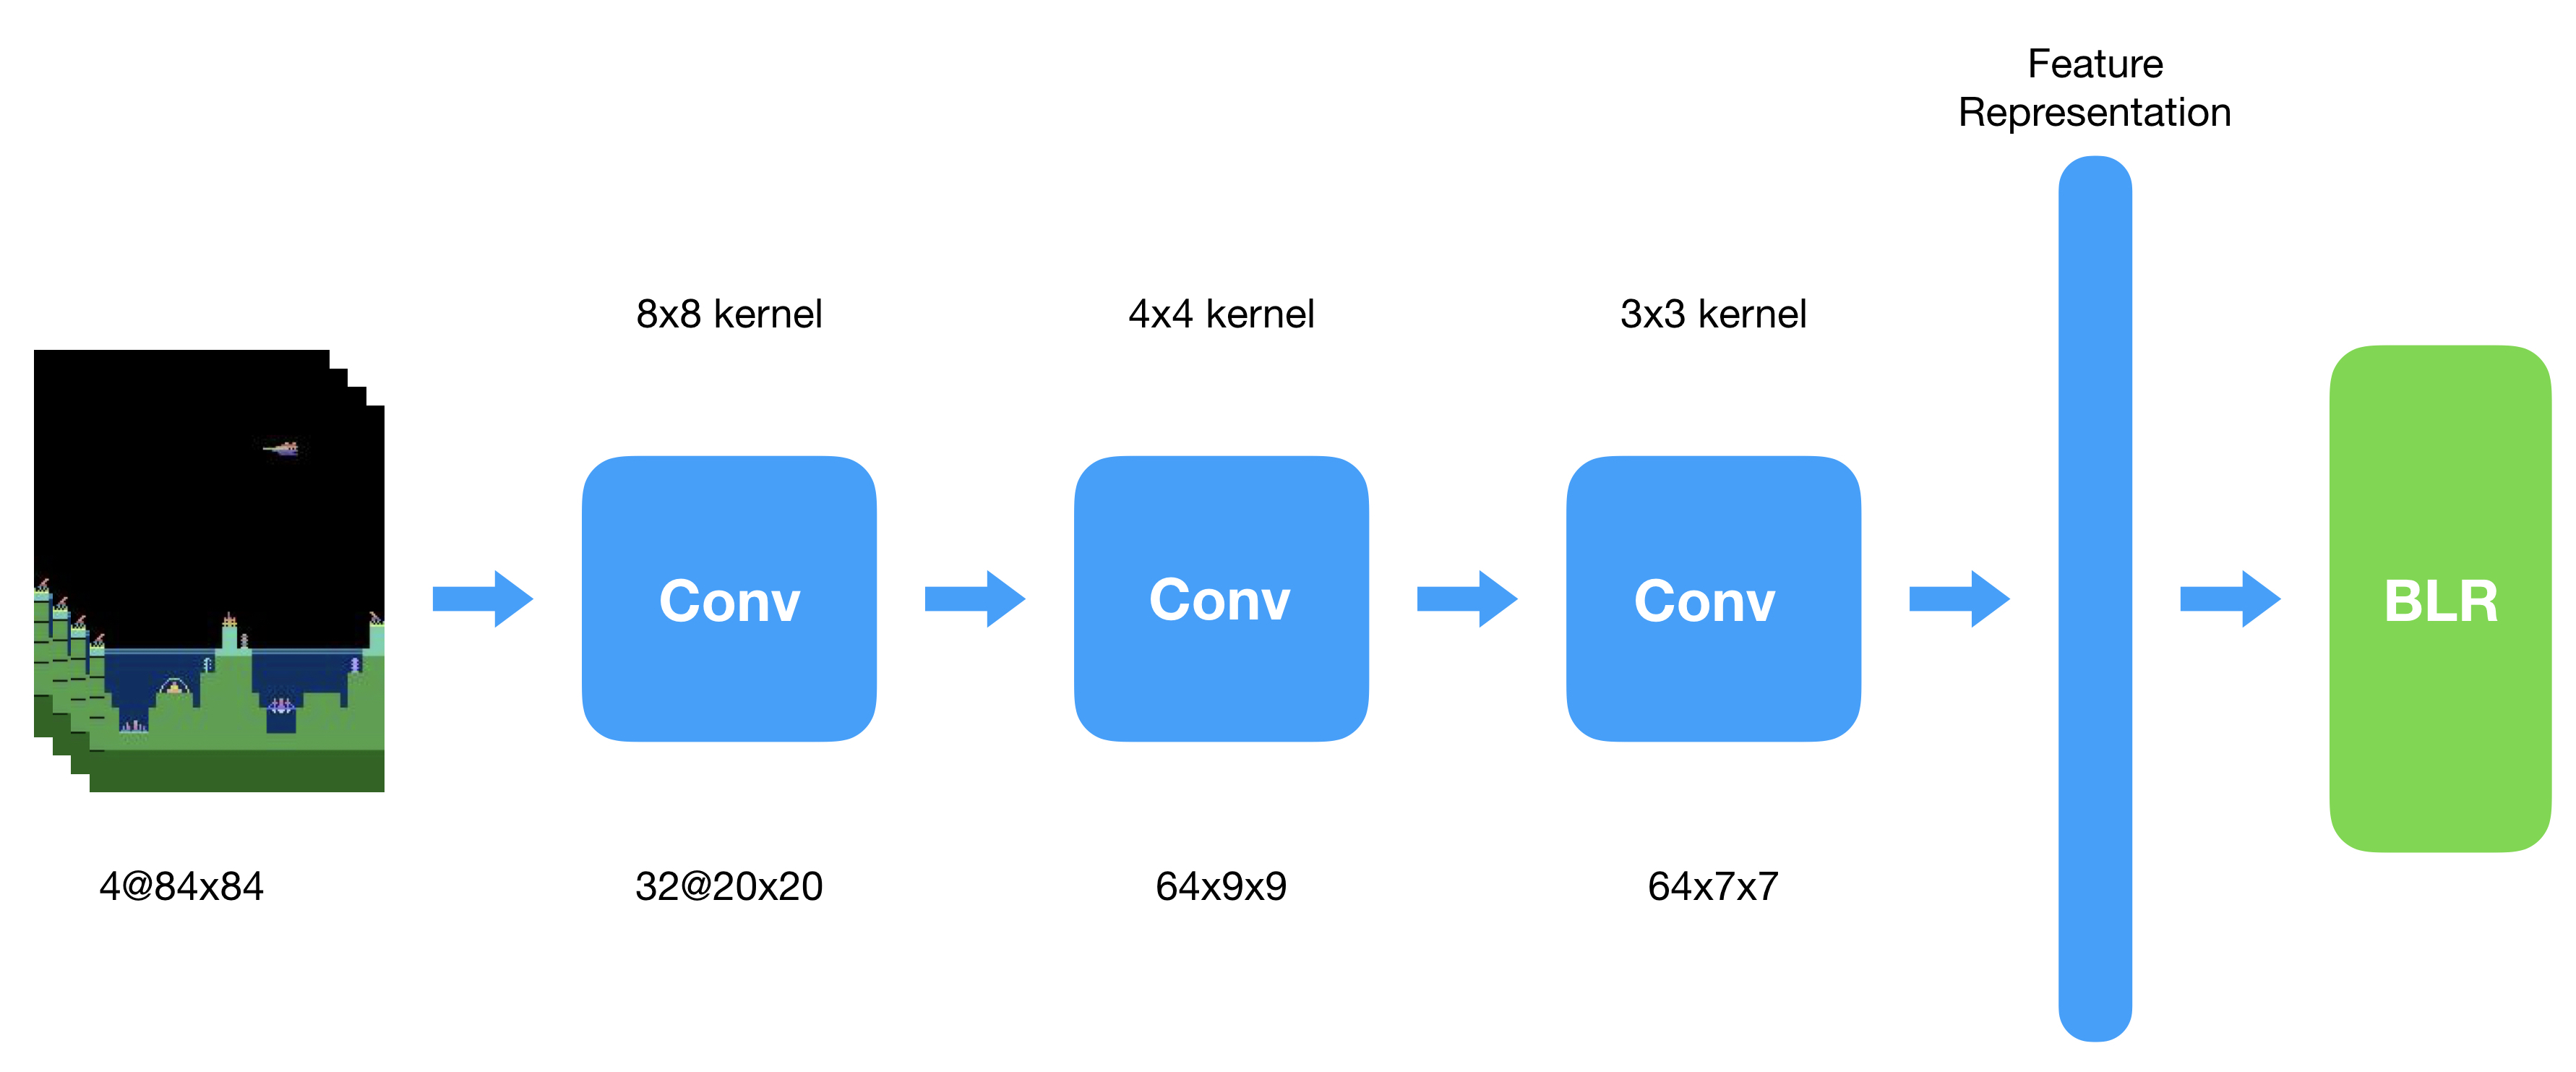
\includegraphics[width=12cm,height=12cm,keepaspectratio]{img/net.jpeg}
\caption{Visual representation of our network design, from \cite{BDQN}}
\end{figure}

\subsection{Output Structure:}
The output of the neural network for a singular $s$ input will be a feature vector $\phi(s)$ of shape $(512)$. For batch input $B_s$ the output will of shape $(|B|,512)$, a matrix composed of $|B| = B_{gd}$ number of $\phi(s)$ vectors for the $s$ in the $B$ batch.

\section{Implementation of the Deep Expected Sarsa Variant}
\begin{enumerate}
    \item We use a $Softmax$ policy instead of $\epsilon$-greedy or greedy policy based on the $argmax$ actions of a $Q$ table or a $Q$ function. \newline\newline \textbf{See: Assistant functions: Policy}
    \item When training the policy network we approximate the expected value of the $Q_{target}(s')$ Q-values at next state by taking the dot product of $M^T\phi_{target}(s')$ with the $Softmax$ function of the next state policy $Q$ values, $Softmax(W^T\phi(s'))$. This value will be used to minimize the Bellman loss, instead of taking $M^T\phi_{target}(s')$ at the coordinate $a = argmax(W^T\phi_{s'})$ as in \cite{EEtBDQN}, which was more of a standard $Q$-learning approach.\newline\newline
    \textbf{See: Training Functions: TrainModel: lines 12-18}
    \item In the case of the posterior update, we take $Softmax(M^T\phi_{target}(s')) \cdot M^T\phi_{target}(s')$ as our 
    expected value estimate, as a replacement for the simpler way of taking the maximum of the $M^T\phi_{target}(s')$ value.\newline\newline
    \textbf{See: Training Functions: PosteriorUpdate: lines 30-36} \newline\newline
    (note that there may be a better way to approximate the expected $Q$-values during both the gradient descent updates of $\phi$ and the posterior updates of $W$)
\end{enumerate}

\clearpage
\section{Bayesian Deep Expected Sarsa Algorithm:}
\begin{algorithm}
    \begin{algorithmic}
    \State \textbf{\underline{Main loop}}
        \State Initialize: $\theta$, $\theta_{target}$, $W$, $M$, $\Sigma$, $L$, $\phi\phi^T$, $\phi_Y$
        \State $RM = \{\}$
        \For {\(1,\dots,N\)}
            \State $ fr \gets reset\;environment$
            \State $ s \gets$ Preprocess($fr$)
            \State \textbf{repeat}
                \State $a \gets$ Policy($s$, $W$)
                \State $s',\;a,\;r,\;d$ $\gets$ Act($a$, $s$)
                \State record $(s,\;a,\;s',\;r,\;d)$ to $RM$
                \State $s \gets s'$
                \State $t_{total}$ += 1
                \If{$t_{total}$ mod $F_1$ $=$ $0$}
                    \State $W \gets$ ThompsonSample()
                \EndIf
                \If{$t_{total}$ mod $F_2$ $=$ $0$}
                    \State TrainModel()
                \EndIf
                \If{$t_{total}$ mod $F_3$ $=$ $0$}
                    \State UpdateTargetNetwork()
                    \If{$t_{total}$ mod $F_4$ $=$ $0$}
                        \State $M$, $\Sigma$ $\gets$ PosteriorUpdate()
                        \For {a = 0,1,2,$\dots$,|A|-1}
                            \State$L_a =$ $Cholesky(\frac{\Sigma_a + \Sigma_a^T}{2})$
                        \EndFor
                    \EndIf
                \EndIf
            \State \textbf{until episode end}
        \EndFor
    \end{algorithmic}[1]
\end{algorithm}
\begin{algorithm}
    \begin{algorithmic}[2]
    \State \textbf{\underline{Assistant Functions:}}
    \State
    \State \underline{Policy($s$,$W$):}
        \State $Q(s) \gets W^T \phi(s)$
        \State $a \sim$ Softmax($Q(s)$)
        \State Return $a$
    \State
    \State
    \State \underline{Preprocess($s$,$fr$):}
        \State $tfr \gets$ transform $fr$ to $84\times84$
        \If{$fr$ is the initial frame}
            \State Return $[tfr,\;tfr,\;tfr,\;tfr]$
        \Else
            \State Return $[s[2],s[3],s[4],tfr]$
        \EndIf
    \State
    \State
    \State \underline{Act($a$, $s$):}
        \State $Cr \gets 0$
        \If{Frame skipping}
            \For{1,\dots,$FR_{skipped}\;+\;1$}
                \State step in the environment with $a$
                \State observe $fr,\;a,\;r,\;d$ after step
                \State $\sum{r'}$ += $r$
            \EndFor
        \ElsIf{No frame skipping}
            \State step from $s$ with $a$
            \State observe $fr,\;a,\;r,\;d$ after step
            \State $\sum{r'}$ += $r$
        \EndIf
    \State
    \State
        \State $s \gets$ Preprocess($s$,$fr$)
        \State Return $s$, $a$, $\sum{r'}$, $a'$
    \State
    \State
    \State \underline{ThompsonSample():}
        \State $Z \sim \mathcal{N}(0,1,512)$ vector of 512 independent samples from $\mathcal{N}(0,1)$ 
        \State $W = M + LZ$
        \State Return $W$
        \end{algorithmic}[2]
\end{algorithm}

\begin{algorithm}
    \begin{algorithmic}[3]
    \State \textbf{\underline{Training Functions}}
    \State
    \State \underline{TrainModel():}
        \State $B \gets$ sample $|B| = B_{post}$ from $RM$
        \State
        \State $B_s,\;B_{s'},\;B_{a},\;Br,\;Bd= \; B$
        \State
        \State $Q(B_s,B_{a}) \gets W_{B_{a}}^T\phi(B_s)$
        \State
        \State $Q(B_{s'}) \gets$ $M^T\phi_{target}(B_{s'})$
        \State
        \State $Probs \gets Softmax( W^T\phi(B_{s'}))$
        \State  
        \State $EQ(B_{s'}) \gets Q(B_{s'})^T \cdot Probs$
        \State
        \State $Loss = MSE(Q(B_s,B_{a}), Br + (1-Bd)\cdot \gamma \cdot EQ(B_{s'}))$
        \State
        \State $\theta \gets Adam(Loss, LR, \theta)$ as a single gradient descent step
    \State
    \State 
    \State \underline{UpdateTargetNetwork():}
        \State $\theta_{target} \gets \theta$
    \State
    \State 
    \State \underline{PosteriorUpdate():}
        \For{1,$\dots$,PosteriorBatchSize}
            \State $B \gets$ sample $|B|=1$ from $RM$
            \State $s,\;s',\;a,\;r\;d = \; B$
            \State
            \State $\phi\phi^T_a \gets \phi\phi^T_a + \phi(s) \phi(s)^T$
            \State
            \State $Q(s') \gets M^T\phi_{target}(s')$
            \State
            \State $EQ(s') \gets Q(s')^T \cdot Softmax(Q(s'))$
            \State
            \State $\phi_{Y_a}\gets \phi_{Y_a} + \phi(s)^T (r + (1 - d) \cdot \gamma \cdot EQ(s'))$
        \EndFor
        \For{a = 0,$\dots$,|A|-1}
            \State $inv \gets (\frac{\phi\phi^T_a}{\sigma_n}  + \frac{1}{\sigma} \cdot I)^{-1}$
            \State
            \State $M_a \gets \frac{inv \cdot \phi_{Y_a}}{\sigma_n}$
            \State
            \State $\Sigma_a \gets \sigma \cdot inv$
        \EndFor
        \State Return $M$, $\Sigma$
    \end{algorithmic}[3]
\end{algorithm}

\clearpage
\section{Limitations}
\begin{enumerate}
    \item The feature extraction convolutional neural network $\phi$ might be oversimplified.
    \item Image downscaling and grayscaling, automatic frameskipping of four frames between two adjacent time steps in the v5 Atari Game environments, and the absence of upsampling layers may cause loss of important information.
    \item Replay memory and posterior update batch size requires a lot of memory.
    \item Sparse and computationally expensive posterior updates.
    \item Hyper parameters such as the four frequencies $F_1,\;F_2,\;F_3,\;F_4$, or the learning rates $\gamma,\; LR$ are likely to be heavily dependent on $env$.
    \item Due to the insufficiency of our budget, we are unfortunately unable to harness the computing power of state-of-the-art GPUs to perform the exhaustive and time-consuming experiments.
\end{enumerate}

\clearpage
\section{Results:}
\begin{enumerate}
    \item We host our code implementation, \textit{.csv} files describing the experiment results, and the plots at \url{https://github.com/Orthologues/DM887-ReinforcementLearning/tree/main/final_project/zhao_BDQN}. Our source code is implemented in a modulized manner.
    \item The $config.py$ files for each of the learning curves shown at \textbf{Figure \ref{fig:pong_learning}} and \textbf{Figure \ref{fig:breakout_learning}} are available publicly at \url{https://github.com/Orthologues/DM887-ReinforcementLearning/blob/main/final_project/zhao_BDQN/test_results/pong-v5_test1/config.py}, \url{https://github.com/Orthologues/DM887-ReinforcementLearning/blob/main/final_project/zhao_BDQN/test_results/pong-v5_test2/config.py}, \url{https://github.com/Orthologues/DM887-ReinforcementLearning/blob/main/final_project/zhao_BDQN/test_results/breakout-v5_test1/config.py}, and \url{https://github.com/Orthologues/DM887-ReinforcementLearning/blob/main/final_project/zhao_BDQN/test_results/breakout-v5_test2/config.py}.
    \item In three out of the four learning curves as shown at \textbf{Figure \ref{fig:pong_learning}} and \textbf{Figure \ref{fig:breakout_learning}}, learning was only slightly achieved after a large number of gradient descent time steps (see section "The state of the art"). Meanwhile, a learning curve using a lower-than-default frequency of gradient descent of $\phi$, and a higher-than-default frequency of target and posterior update at $env2$ failed to learn, which is indicated by the negative slope of the linear regression line.
    \item As shown at \textbf{Figure \ref{fig:pong_learning}}, increasing $LR$ (default = 0.0025) of the gradient descent update of $\phi$ to 0.01 has non-observable effects on the learning curve.
    \item As shown at \textbf{Figure \ref{fig:breakout_learning}}, using a higher-than-default frequency for $W_{target}$ update (default = $F_3$) and posterior update (default = $F_3 \times F_4$) culminates in a negative learning curve.
    \item As shown at \textbf{Figure \ref{fig:breakout_learning}}, using a lower-than-default frequency for $\phi$ update (default = $F_2$) culminates in a negative learning curve.
\end{enumerate}

\begin{figure} [ht]
    \centering
    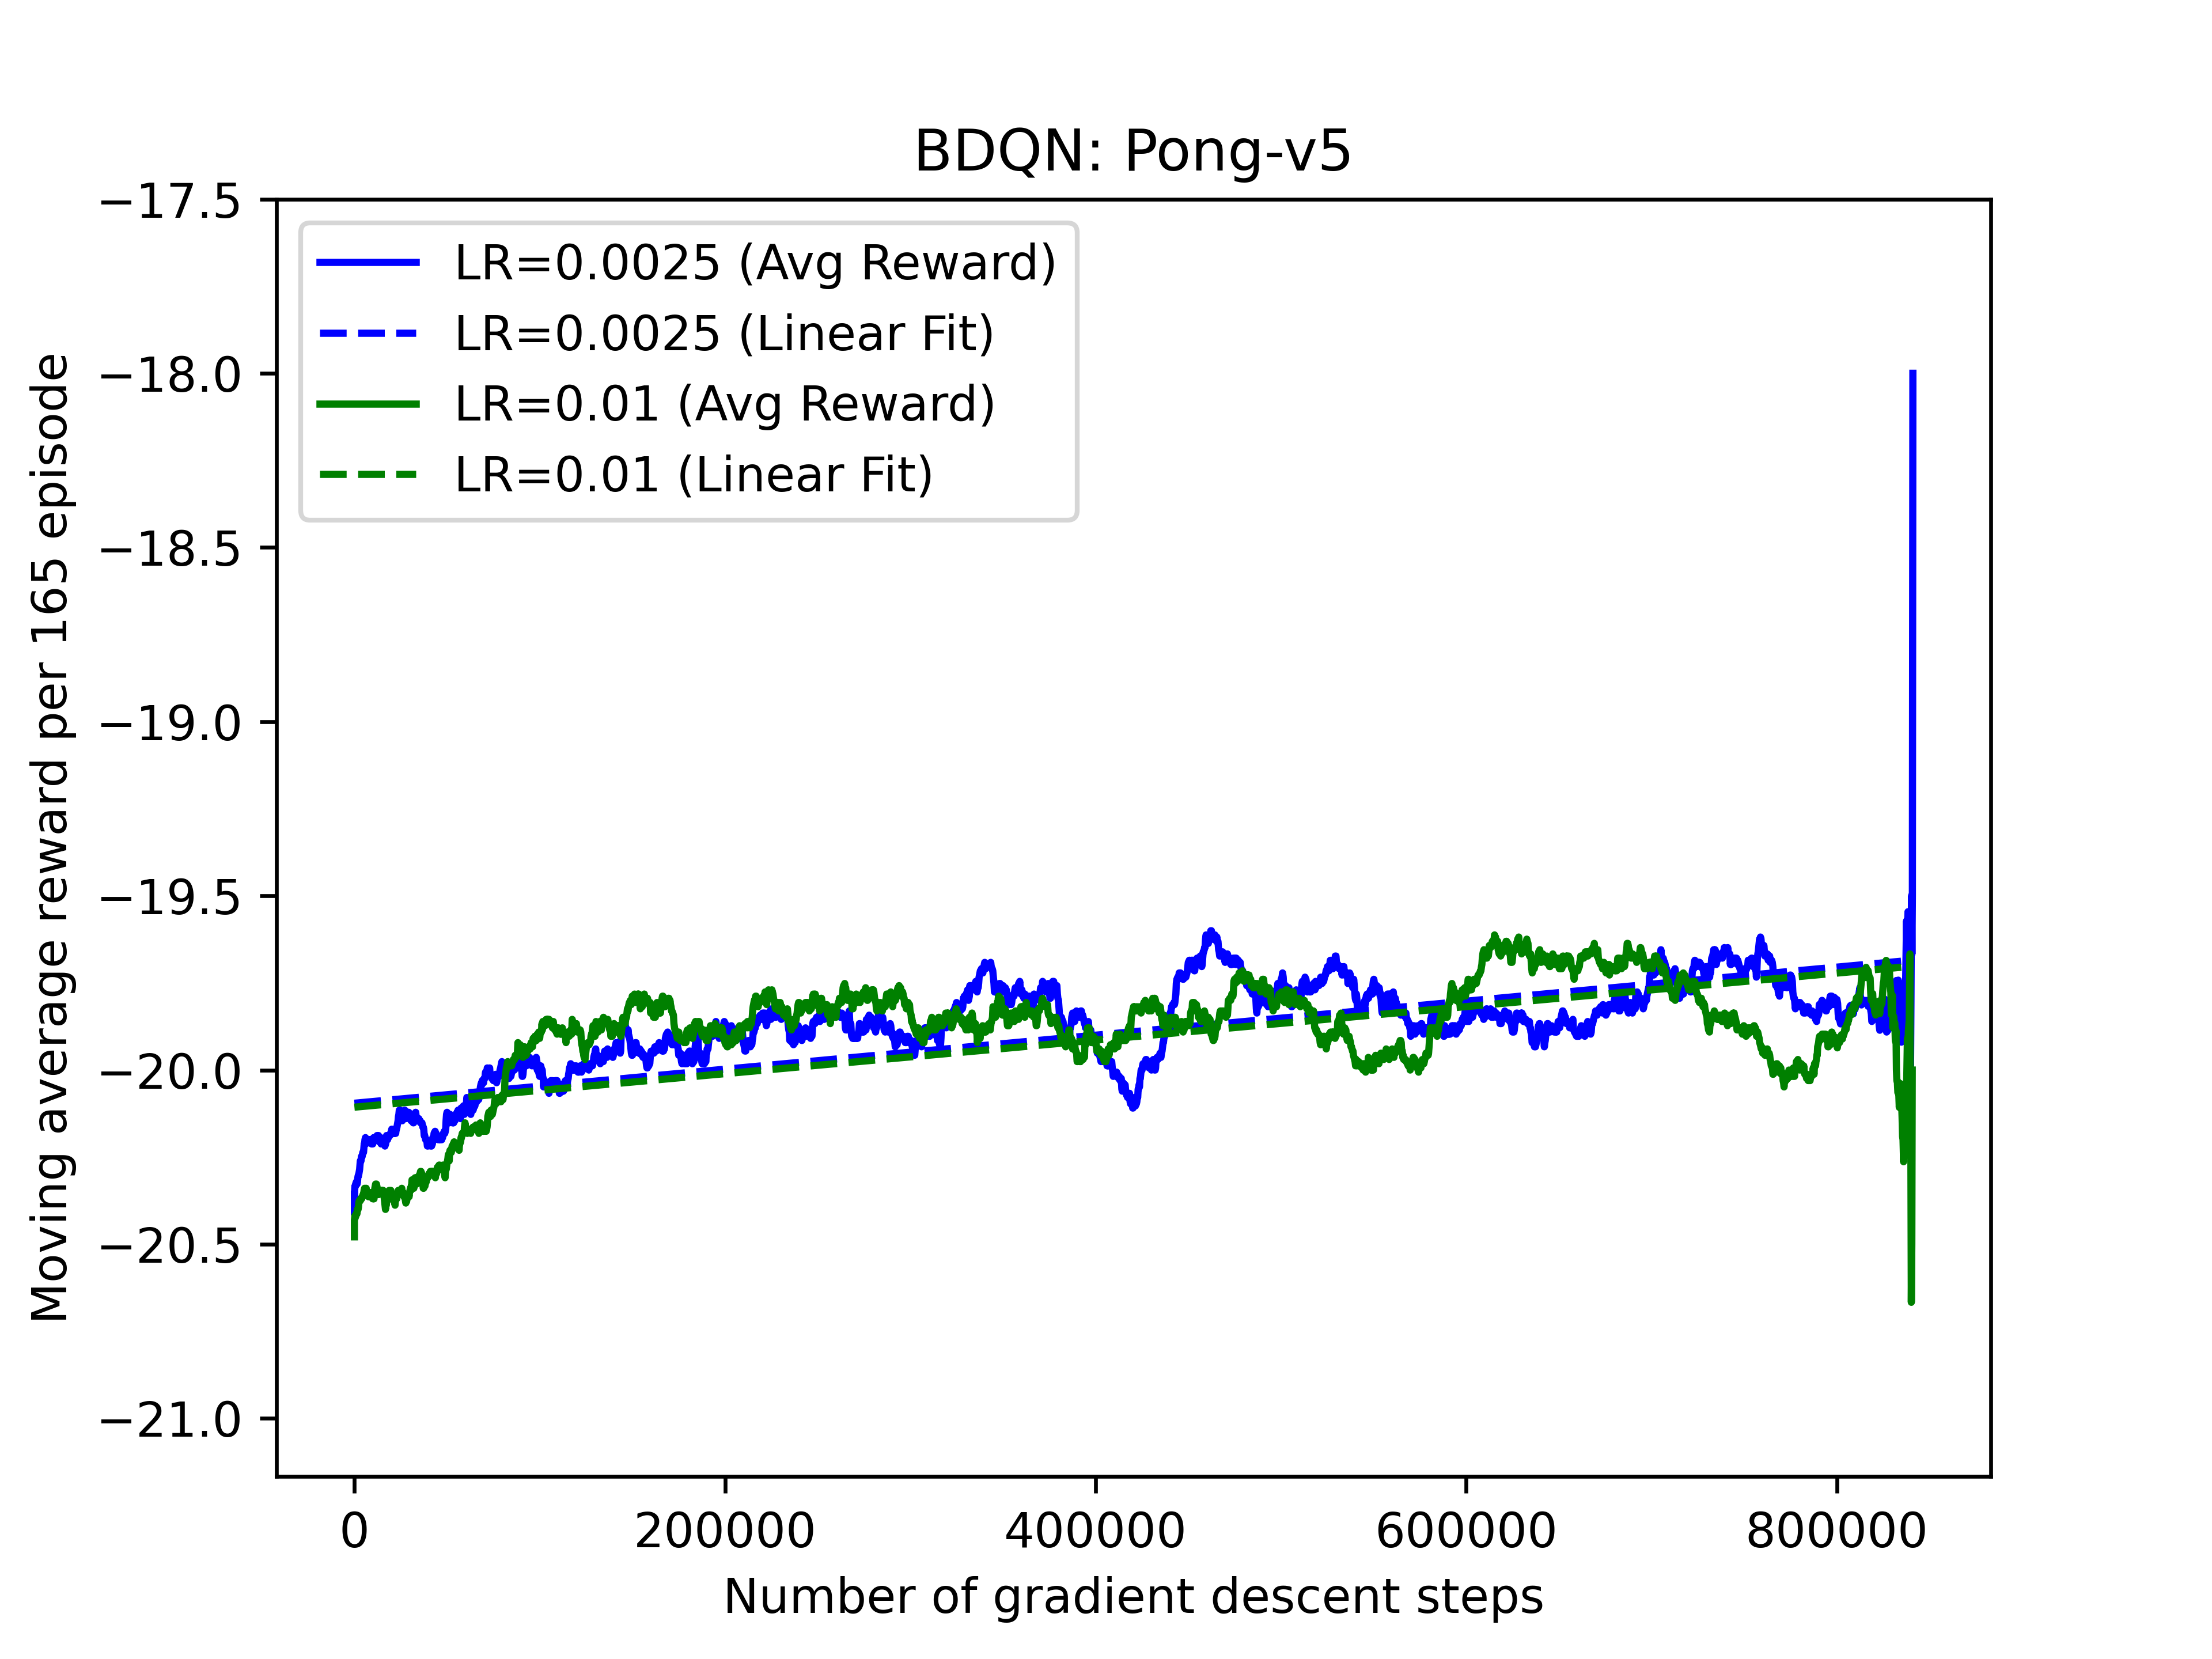
\includegraphics[width=1\textwidth]{img/pong-v5_learning.png}
    \caption{Learning at \textbf{\textit{env1}}}
    \label{fig:pong_learning}
\end{figure}

\begin{figure} [ht]
    \centering
    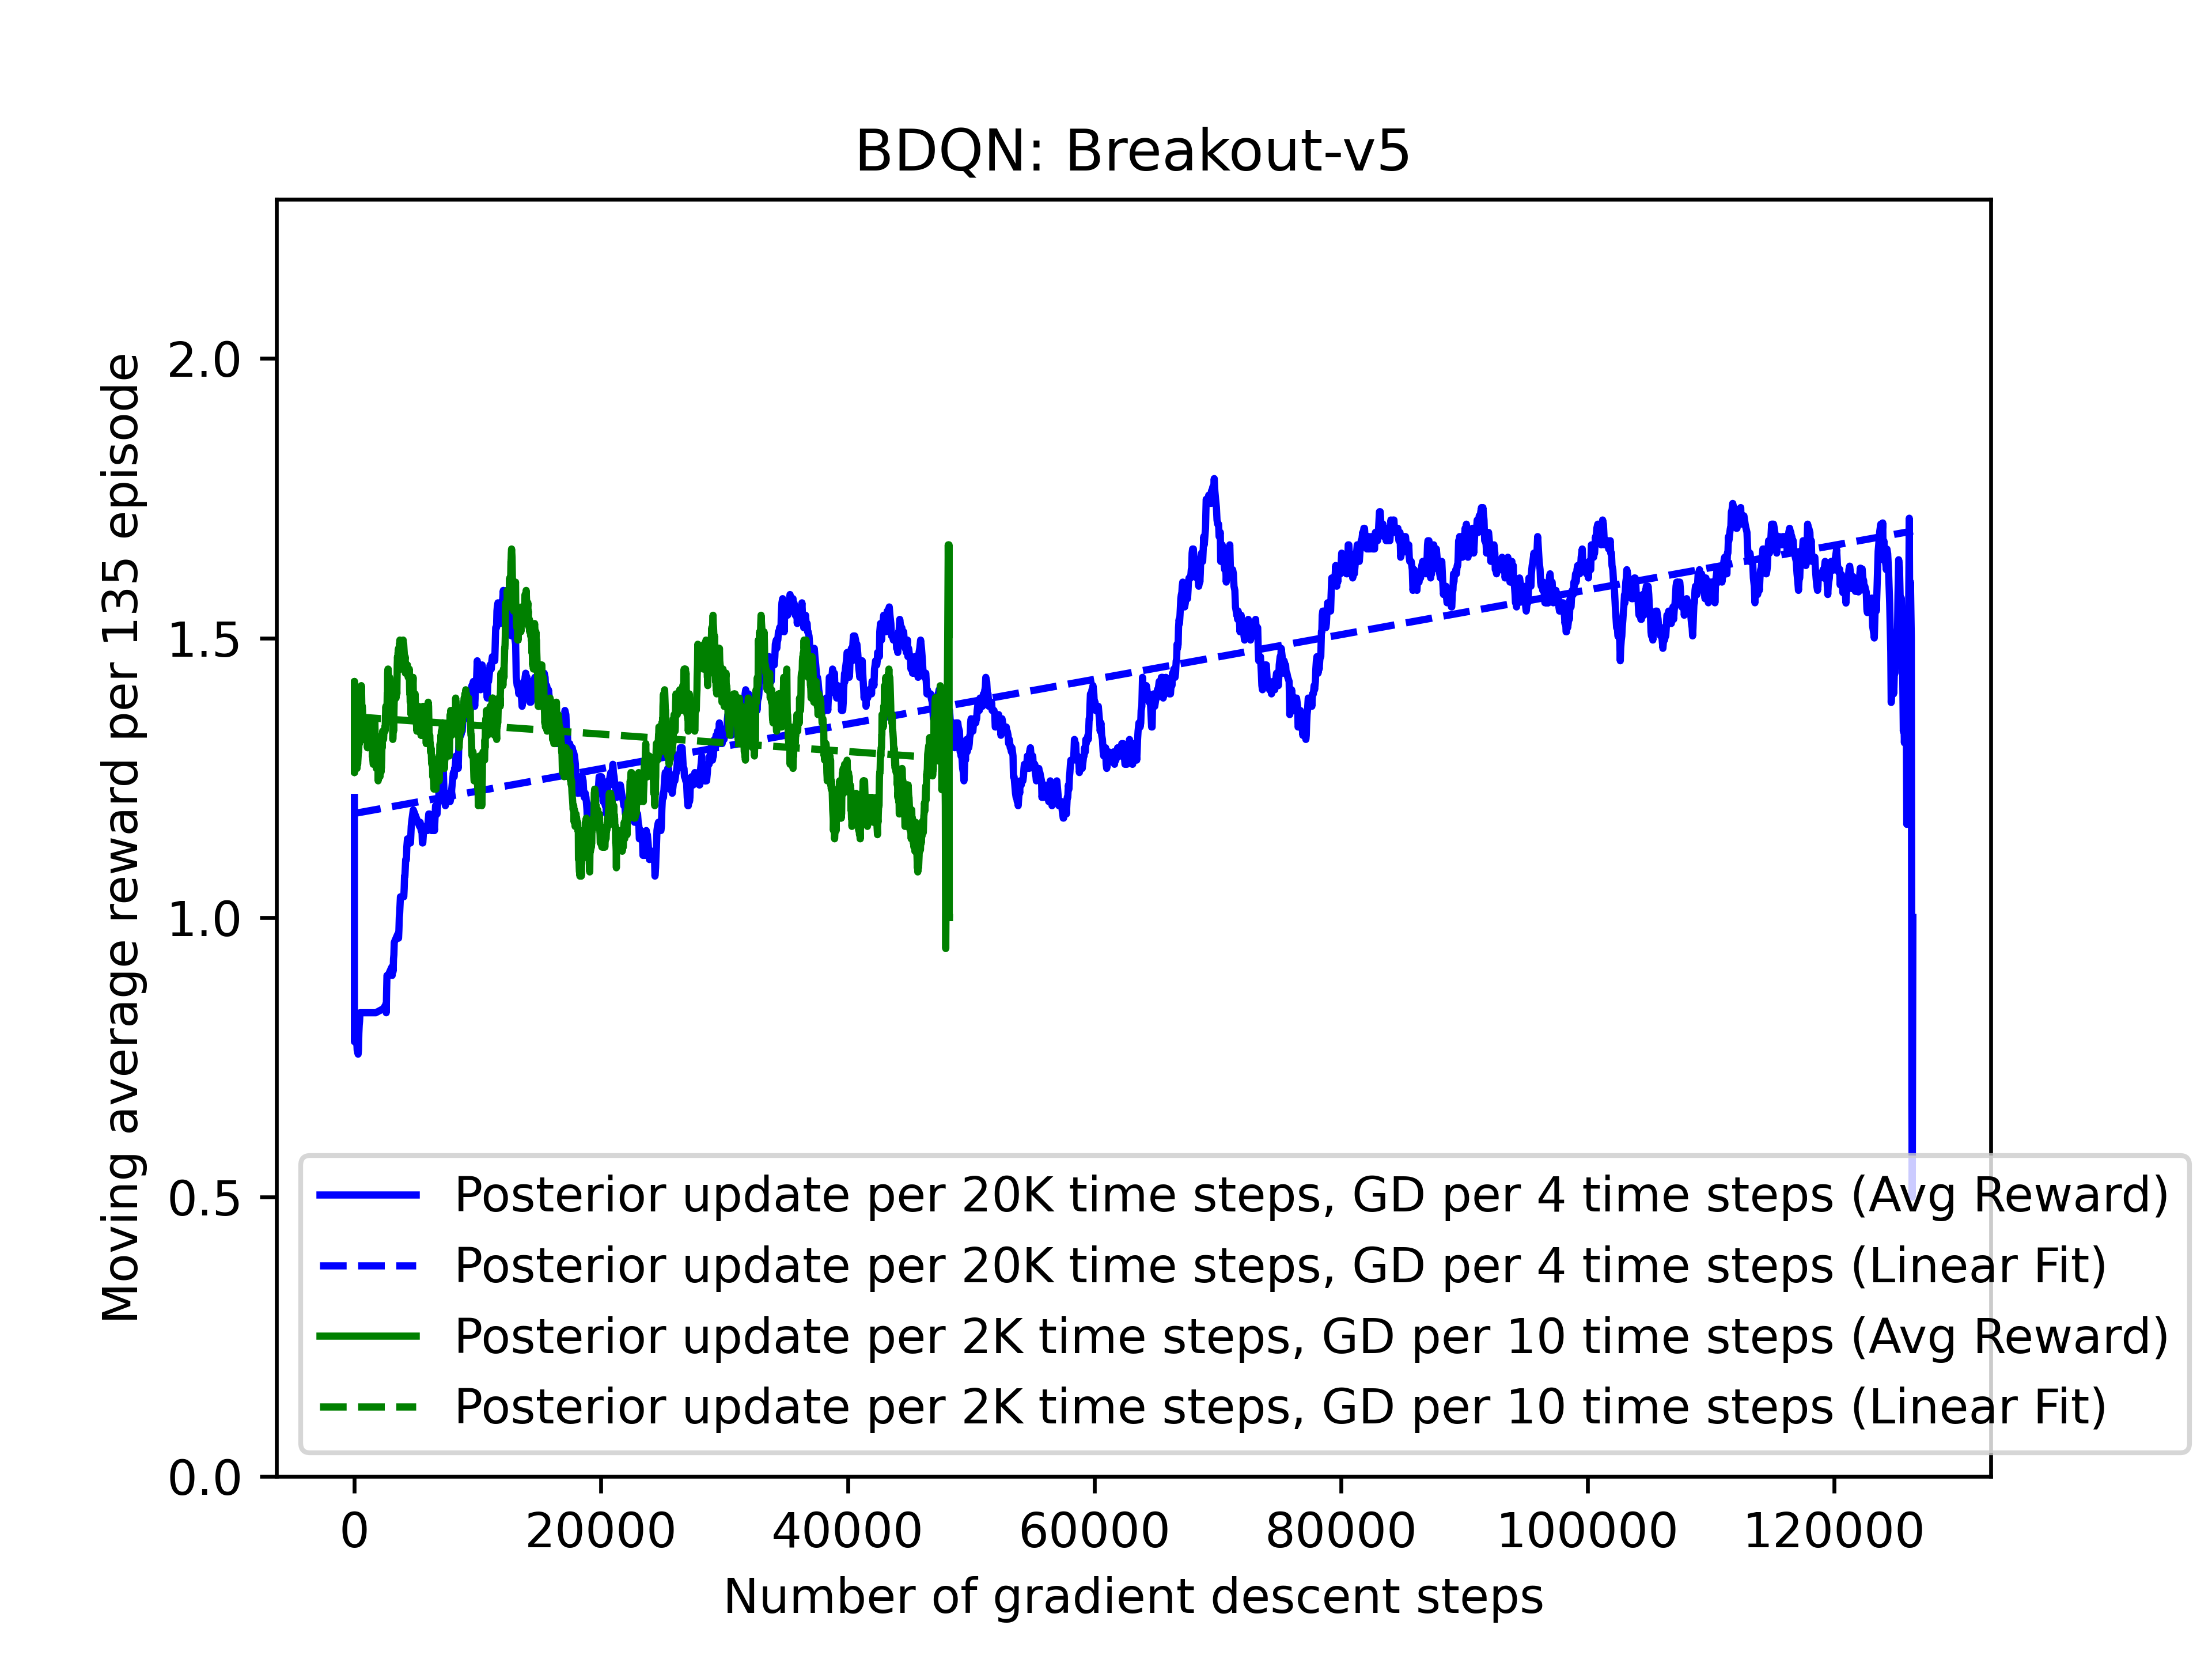
\includegraphics[width=1\textwidth]{img/breakout-v5_learning.png}
    \caption{Learning at \textbf{\textit{env2}}}
    \label{fig:breakout_learning}
\end{figure}

\clearpage
\section{The state of the art}
One of the main reasons we decided to follow \cite{BDQN} and \cite{EEtBDQN} was that they performed well documented training sessions. In these experiments they achieved very good results, although only after training for far more episodes than we were able to.

\begin{figure}[H]
\centering
\begin{subfigure}{.5\textwidth}
  \centering
  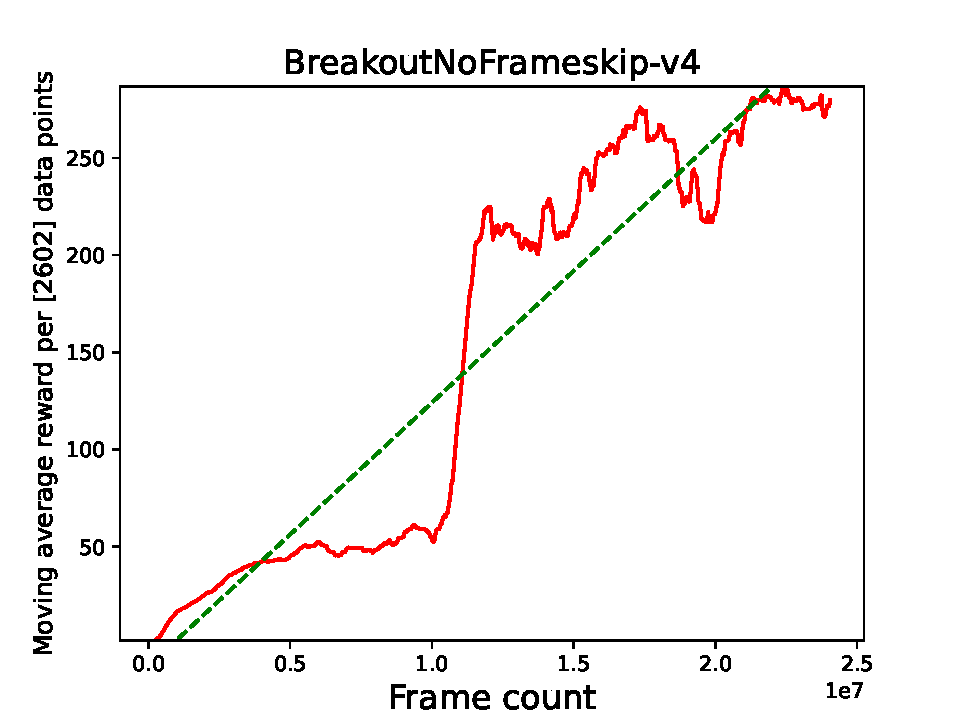
\includegraphics[width=7cm,height=7cm,keepaspectratio]{img/BreakoutNoFrameskipv4.pdf}
  \caption{Results from \cite{BDQN}, on the Breakout environment, plotted with our averaging algorithm.}
  \label{fig:sub1}
\end{subfigure}%
\begin{subfigure}{.5\textwidth}
  \centering
  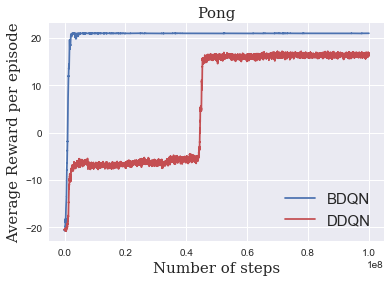
\includegraphics[width=7cm,height=7cm,keepaspectratio]{img/Pong.png}
  \caption{Results from \cite{BDQN}, on the Pong environment.}
  \label{fig:sub2}
\end{subfigure}
\caption{Their model was able to produce fairly good results after around 1 million steps in both environments, and really good ones after $10$ and $100$ million steps. We have only ran our algorithms for at most a few million steps, however we couldn't come close to even an average reward of 20. We don't have any information about the exact hyperparameters used for these tests, which could be bring our algorithm to similar learning speeds as well.}
%\label{fig:test}
\end{figure}

In the \cite{BDQN} project, they compared the BDQN algorithm to DDQN, as it can be observed in their plots. They have found the BDQN to work better on Atari game environments. We have also found sources trying with the DQN algorithm \cite{DQN}.

\begin{figure}[H]
    \centering
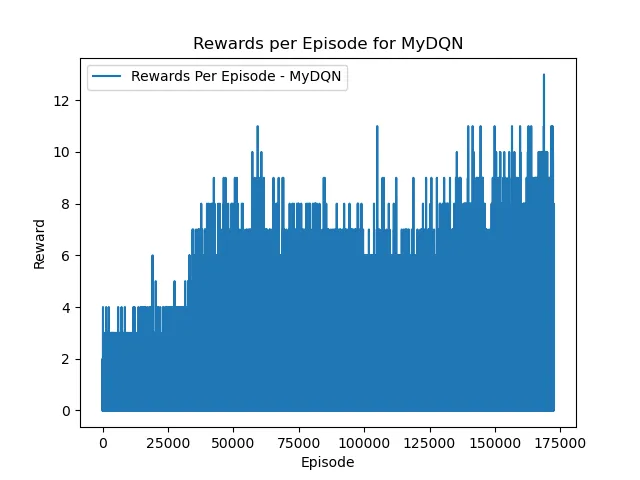
\includegraphics[width=10cm,height=10cm,keepaspectratio]{img/1.png}
\caption{Results of \cite{DQN} on the Breakout environment. Original caption: "MyDQN on Breakout after 10 million steps which corresponds roughly to 175000 episodes".}
\end{figure}

The DQN approach seem to have resulted in much less success than the more advanced techniques. This result is the most comparable to our own, as after 10 million steps of training, at around 5 times more than what we were able to train, their maximal reward doesn't exceed what we observed in our experiments.
\newline\newline
We have found trials with a much more complex neural network structures as well, which interestingly also use 4 stacked frames as an input.
\begin{figure}[H]
    \centering
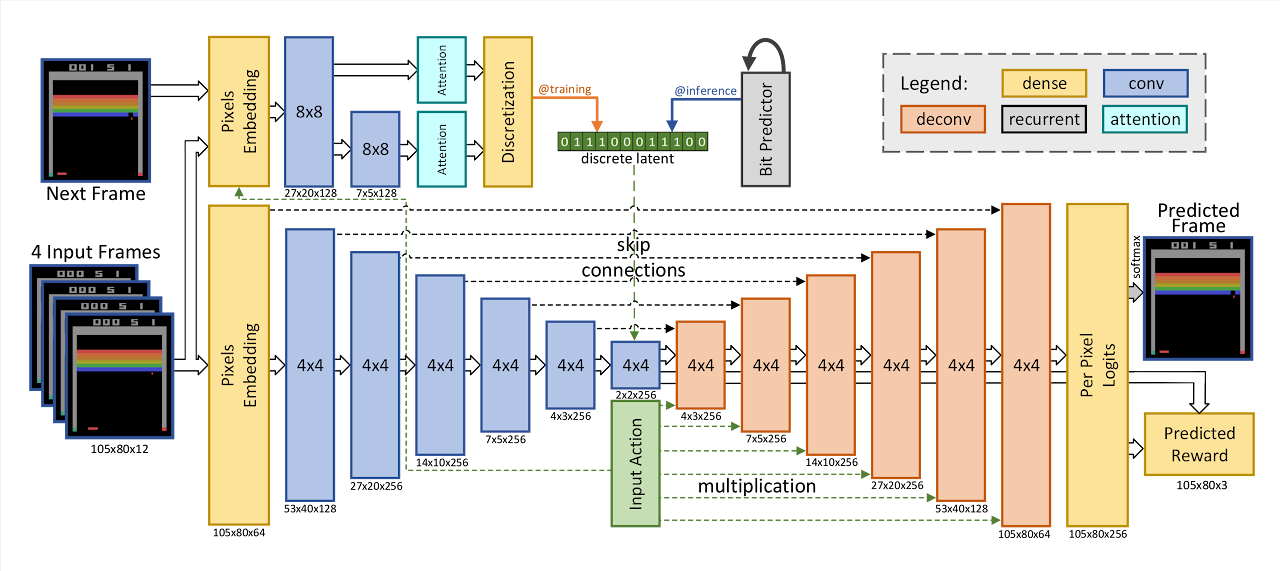
\includegraphics[width=12cm,height=12cm,keepaspectratio]{img/EmbeddedImage.png}
\caption{The neural network structure implemented by \cite{largenet}. They are using a Simulated Policy Learning algorithm and train their policy using the PPO algorithm.}
\end{figure}
Many papers refer to the Rainbow algorithm \cite{rainbow} as the "state of the art" when it comes to reinforcement learning on Atari game environments. As it combines many techniques in the field to achieve consistent and fast learning. Interestingly, the Breakout environment proves difficult for even this algorithm.
\begin{figure}[H]
    \centering
    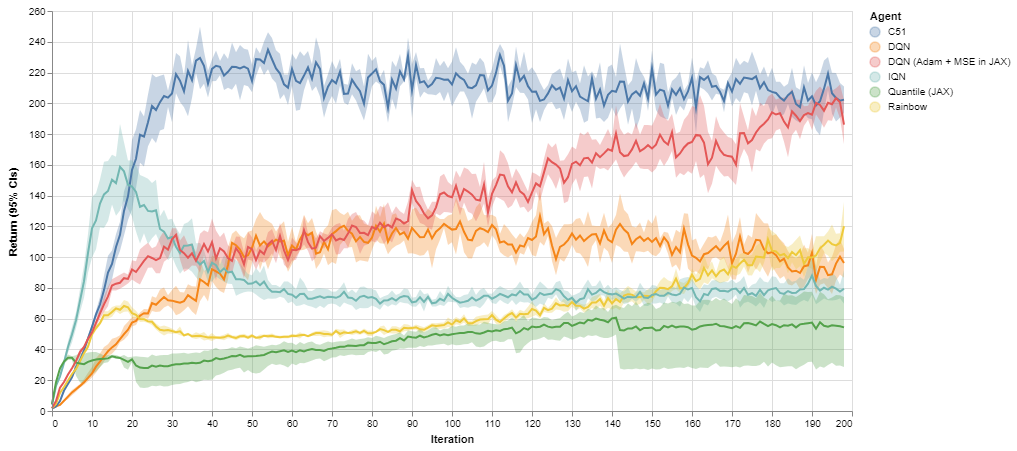
\includegraphics[width=12cm,height=12cm,keepaspectratio]{img/download.png}
\caption{Plot from \cite{plots}. Results on the Breakout environment. Each iteration stands for 250000 steps.}
\end{figure}
\begin{figure}[H]
    \centering
    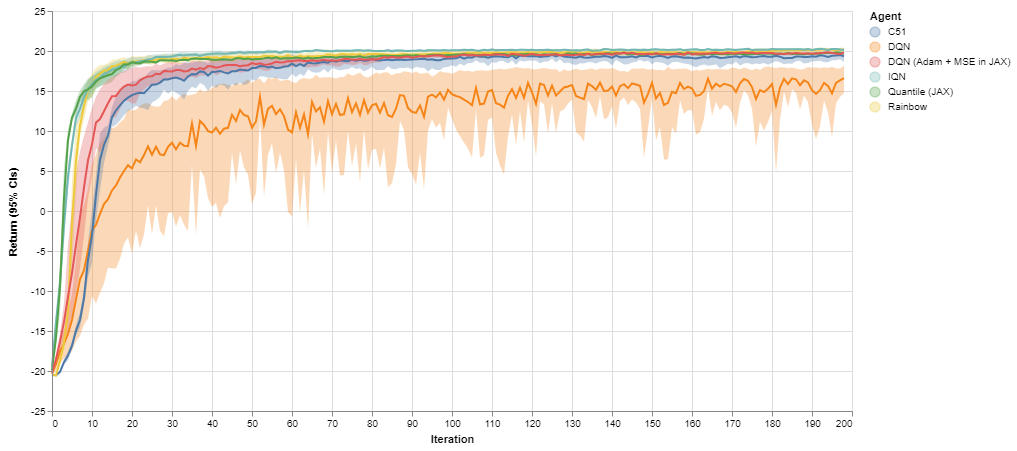
\includegraphics[width=12cm,height=12cm,keepaspectratio]{img/pong2.png}
\caption{Plot from \cite{plots}. Results on the Pong environment. Each iteration stands for 250000 steps.}
\end{figure}
These plots from \cite{plots} show the performance of several reinforcement learning algorithms on the Breakout (top) and Pong (bottom) environments. It is clear that for even the best algorithms, many millions of steps are required to achieve high rewards. 

\clearpage
\begin{thebibliography}{99}

\bibitem{Gym}
\emph{Gymnasium Atari Environments} \url{https://gymnasium.farama.org/environments/atari/}

\bibitem{BDQN}
\emph{BDQN Repository} \url{https://github.com/kazizzad/BDQN-MxNet-Gluon/blob/master/BDQN.ipynb}
\newline
\bibitem{EEtBDQN}
\emph{Efficient Exploration through Bayesian Deep Q-Networks} \url{https://arxiv.org/pdf/1802.04412}
\bibitem{DQN}
\emph{Playing Atari games with Deep Reinforcement Learning and Attention} \url{https://medium.com/@mboungoucolombe/playing-atari-games-with-deep-reinforcement-learning-and-attention-d83312fe4f29}
\bibitem{largenet}
\emph{Model-Based Reinforcement Learning for Atari} \url{https://sites.google.com/view/modelbasedrlatari/home}
\bibitem{rainbow}
\emph{Rainbow: Combining Improvements in Deep Reinforcement Learning} \url{https://arxiv.org/pdf/1710.02298}
\bibitem{plots}
\emph{Baseline plots} \url{https://google.github.io/dopamine/baselines/atari/plots.html}

\end{thebibliography}

\end{document}
